\documentclass[11pt,letterpaper]{article}

\newcommand{\manualTitulo}{Manual del Auditor}
\newcommand{\manualPerfil}{Auditor / Inspector de Cumplimiento}
\newcommand{\manualRol}{AUDITOR}
\newcommand{\usuarioNombre}{Auditor Hernández}
\newcommand{\usuarioEmail}{auditor@pharma.com}

% Estilo compartido de los manuales de PharmaWeigh.
% Cada manual lo carga con % Estilo compartido de los manuales de PharmaWeigh.
% Cada manual lo carga con % Estilo compartido de los manuales de PharmaWeigh.
% Cada manual lo carga con \input{pharma_estilo} y define antes
% \manualTitulo, \manualPerfil, \manualRol.
% Compilar con xelatex (fuentes por fontspec).
\usepackage[T1]{fontenc}
\usepackage[utf8]{inputenc}
\usepackage[spanish,es-tabla,es-noindentfirst]{babel}
\usepackage{lmodern}
\renewcommand*\familydefault{\sfdefault}
\usepackage{geometry}
\usepackage{graphicx}
\usepackage{xcolor}
\usepackage{tabularx}
\usepackage{array}
\usepackage{booktabs}
\usepackage{ragged2e}
\usepackage{enumitem}
\usepackage{tcolorbox}
\usepackage{fancyhdr}
\usepackage{hyperref}
\usepackage{tikz}
\usetikzlibrary{positioning, arrows.meta, shapes.geometric}

\geometry{letterpaper, top=2.4cm, bottom=2cm, left=2cm, right=2cm}
\setlength{\headheight}{34pt}
\addtolength{\topmargin}{-12pt}

% ── Paleta PharmaWeigh ──────────────────────────────────────────────
\definecolor{pharmaazul}{HTML}{1E40AF}      % acento principal
\definecolor{pharmablue}{HTML}{2563EB}       % botones y highlights
\definecolor{pharmalight}{HTML}{3B82F6}      % links y secundarios
\definecolor{pharmagreen}{HTML}{16A34A}      % éxito / aprobado
\definecolor{pharmayellow}{HTML}{D97706}     % advertencia / cuarentena
\definecolor{pharmared}{HTML}{DC2626}        % error / rechazado / peligro
\definecolor{pharmaslate}{HTML}{1E293B}      % sidebar / fondo oscuro
\definecolor{tinta}{HTML}{0F172A}            % texto principal
\definecolor{grisfondo}{HTML}{F1F5F9}        % fondo claro
\definecolor{gristexto}{HTML}{64748B}        % texto secundario
\definecolor{grislinea}{HTML}{CBD5E1}        % líneas y bordes

\hypersetup{colorlinks=true, linkcolor=pharmalight, urlcolor=pharmalight}

% ── Header / Footer ────────────────────────────────────────────────
\pagestyle{fancy}
\fancyhf{}
\fancyhead[L]{%
    \raisebox{-4pt}{\tikz\draw[fill=pharmablue,draw=none,rounded corners=3pt]
        (0,0) rectangle (0.7cm,0.7cm)
        node[midway,white,font=\bfseries\footnotesize] {PW};}%
    \hspace{6pt}\footnotesize\color{gristexto}\textbf{PharmaWeigh}}
\fancyhead[R]{\footnotesize\color{gristexto}\manualTitulo\ --- \manualPerfil}
\fancyfoot[C]{\footnotesize\color{gristexto}\thepage}
\renewcommand{\headrulewidth}{0.6pt}
\renewcommand{\headrule}{\hbox to\headwidth{%
    \color{pharmaazul}\leaders\hrule height \headrulewidth\hfill}}

% ── Secciones ───────────────────────────────────────────────────────
\newcommand{\seccion}[1]{%
    \vspace{4pt}
    {\large\bfseries\color{tinta}#1}\par\vspace{2pt}
    {\color{pharmaazul}\rule{\linewidth}{1.2pt}}\par
    \vspace{6pt}
}
\newcommand{\subseccion}[1]{%
    \vspace{8pt}
    \noindent{\bfseries\color{pharmaslate}#1}\par
    \vspace{3pt}
}

% ── Cajas de aviso ──────────────────────────────────────────────────
\newtcolorbox{cajaNota}{
    colback=grisfondo, colframe=gristexto!50, rounded corners,
    boxrule=1pt, left=10pt, right=10pt, top=6pt, bottom=6pt }
\newtcolorbox{cajaOjo}{
    colback=pharmared!7, colframe=pharmared, rounded corners,
    boxrule=1.2pt, left=10pt, right=10pt, top=6pt, bottom=6pt,
    fontupper=\color{pharmared!80!black} }
\newtcolorbox{cajaInfo}[1][]{
    colback=grisfondo, colframe=pharmaazul, fonttitle=\bfseries\color{white},
    colbacktitle=pharmaazul, title=#1, rounded corners,
    boxrule=1pt, left=8pt, right=8pt, top=6pt, bottom=6pt }
\newtcolorbox{cajaTip}[1][]{
    colback=pharmagreen!6, colframe=pharmagreen, fonttitle=\bfseries\color{white},
    colbacktitle=pharmagreen, title=#1, rounded corners,
    boxrule=1pt, left=8pt, right=8pt, top=6pt, bottom=6pt }
\newtcolorbox{cajaPeligro}[1][MATERIAL PELIGROSO]{
    colback=pharmared!8, colframe=pharmared, fonttitle=\bfseries\color{white},
    colbacktitle=pharmared, title=#1, rounded corners,
    boxrule=1.5pt, left=8pt, right=8pt, top=6pt, bottom=6pt }
\newtcolorbox{cajaCuarentena}[1][CUARENTENA]{
    colback=pharmayellow!8, colframe=pharmayellow, fonttitle=\bfseries\color{white},
    colbacktitle=pharmayellow, title=#1, rounded corners,
    boxrule=1.2pt, left=8pt, right=8pt, top=6pt, bottom=6pt }

% ── Listas ──────────────────────────────────────────────────────────
\setlist[itemize]{leftmargin=16pt, itemsep=3pt, topsep=3pt}
\setlist[enumerate]{leftmargin=20pt, itemsep=5pt, topsep=4pt}
\renewcommand{\arraystretch}{1.3}

% ── Atajos ──────────────────────────────────────────────────────────
\newcommand{\cd}[1]{{\ttfamily\small #1}}
\newcommand{\boton}[1]{{\bfseries\color{pharmablue}[#1]}}
\newcommand{\menu}[1]{{\bfseries\color{pharmaslate}#1}}
\newcommand{\campo}[1]{{\itshape\color{gristexto}#1}}
\newcommand{\codigo}[1]{{\ttfamily\footnotesize\colorbox{grisfondo}{\color{tinta}\,#1\,}}}

% Estados de lote
\newcommand{\aprobado}{{\bfseries\color{pharmagreen}APROBADO}}
\newcommand{\cuarentena}{{\bfseries\color{pharmayellow}CUARENTENA}}
\newcommand{\rechazado}{{\bfseries\color{pharmared}RECHAZADO}}
\newcommand{\agotado}{{\bfseries\color{gristexto}AGOTADO}}

% Estados de orden
\newcommand{\pendiente}{{\bfseries\color{pharmayellow}PENDIENTE}}
\newcommand{\enproceso}{{\bfseries\color{pharmalight}EN PROCESO}}
\newcommand{\dispensado}{{\bfseries\color{pharmagreen}DISPENSADO}}
\newcommand{\completada}{{\bfseries\color{pharmagreen!80!black}COMPLETADA}}

% Semáforo
\newcommand{\semaverde}{\tikz\draw[fill=pharmagreen,draw=pharmagreen!70!black] (0,0) circle (5pt);}
\newcommand{\semaamarillo}{\tikz\draw[fill=pharmayellow,draw=pharmayellow!70!black] (0,0) circle (5pt);}
\newcommand{\semarojo}{\tikz\draw[fill=pharmared,draw=pharmared!70!black] (0,0) circle (5pt);}

% ── Portada ─────────────────────────────────────────────────────────
\newcommand{\portada}[2]{%
\thispagestyle{empty}
\begin{center}
    \vspace*{30pt}
    {\tikz\draw[fill=pharmablue,draw=none,rounded corners=8pt]
        (0,0) rectangle (2cm,2cm)
        node[midway,white,font=\bfseries\Large] {PW};}\\[16pt]
    {\Huge\bfseries\color{tinta}PharmaWeigh}\\[6pt]
    {\large\color{gristexto}Sistema de Control de Producción y Calidad Farmacéutica}\\[20pt]
    {\color{pharmaazul}\rule{0.6\linewidth}{2pt}}\\[20pt]
    {\LARGE\bfseries\color{tinta}\manualTitulo}\\[8pt]
    {\normalsize\color{gristexto}#1}\\[16pt]
    {\large\bfseries\color{pharmaslate}\usuarioNombre}\\[4pt]
    {\normalsize\color{gristexto}Rol: \manualRol}\\[4pt]
    {\footnotesize\color{gristexto}#2}\\[4pt]
    {\footnotesize\color{gristexto}Septiembre de 2026}\\[14pt]
    {\color{pharmaazul}\rule{0.4\linewidth}{1.2pt}}\\[20pt]
    \begin{cajaNota}
    \footnotesize Este documento es confidencial y de uso interno.
    Contiene credenciales personales de acceso al sistema.
    No compartir ni reproducir sin autorización.
    \end{cajaNota}
\end{center}
\newpage }

% ── Tabla de acceso ─────────────────────────────────────────────────
\providecommand{\perfilTexto}{Operario: ejecutas el pesaje y dispensado de materiales.}
\newcommand{\tablaAcceso}{%
\noindent\begin{tabularx}{\linewidth}{@{}>{\raggedright\arraybackslash}p{0.28\linewidth} X@{}}
\toprule
\textbf{URL del sistema} & \cd{https://pharma-formweigh.vercel.app} \\
\textbf{Tu usuario} & \cd{\usuarioEmail} \\
\textbf{Tu contraseña} & \cd{\usuarioClave} \\
\textbf{Tu perfil} & \perfilTexto \\
\bottomrule
\end{tabularx}}
 y define antes
% \manualTitulo, \manualPerfil, \manualRol.
% Compilar con xelatex (fuentes por fontspec).
\usepackage[T1]{fontenc}
\usepackage[utf8]{inputenc}
\usepackage[spanish,es-tabla,es-noindentfirst]{babel}
\usepackage{lmodern}
\renewcommand*\familydefault{\sfdefault}
\usepackage{geometry}
\usepackage{graphicx}
\usepackage{xcolor}
\usepackage{tabularx}
\usepackage{array}
\usepackage{booktabs}
\usepackage{ragged2e}
\usepackage{enumitem}
\usepackage{tcolorbox}
\usepackage{fancyhdr}
\usepackage{hyperref}
\usepackage{tikz}
\usetikzlibrary{positioning, arrows.meta, shapes.geometric}

\geometry{letterpaper, top=2.4cm, bottom=2cm, left=2cm, right=2cm}
\setlength{\headheight}{34pt}
\addtolength{\topmargin}{-12pt}

% ── Paleta PharmaWeigh ──────────────────────────────────────────────
\definecolor{pharmaazul}{HTML}{1E40AF}      % acento principal
\definecolor{pharmablue}{HTML}{2563EB}       % botones y highlights
\definecolor{pharmalight}{HTML}{3B82F6}      % links y secundarios
\definecolor{pharmagreen}{HTML}{16A34A}      % éxito / aprobado
\definecolor{pharmayellow}{HTML}{D97706}     % advertencia / cuarentena
\definecolor{pharmared}{HTML}{DC2626}        % error / rechazado / peligro
\definecolor{pharmaslate}{HTML}{1E293B}      % sidebar / fondo oscuro
\definecolor{tinta}{HTML}{0F172A}            % texto principal
\definecolor{grisfondo}{HTML}{F1F5F9}        % fondo claro
\definecolor{gristexto}{HTML}{64748B}        % texto secundario
\definecolor{grislinea}{HTML}{CBD5E1}        % líneas y bordes

\hypersetup{colorlinks=true, linkcolor=pharmalight, urlcolor=pharmalight}

% ── Header / Footer ────────────────────────────────────────────────
\pagestyle{fancy}
\fancyhf{}
\fancyhead[L]{%
    \raisebox{-4pt}{\tikz\draw[fill=pharmablue,draw=none,rounded corners=3pt]
        (0,0) rectangle (0.7cm,0.7cm)
        node[midway,white,font=\bfseries\footnotesize] {PW};}%
    \hspace{6pt}\footnotesize\color{gristexto}\textbf{PharmaWeigh}}
\fancyhead[R]{\footnotesize\color{gristexto}\manualTitulo\ --- \manualPerfil}
\fancyfoot[C]{\footnotesize\color{gristexto}\thepage}
\renewcommand{\headrulewidth}{0.6pt}
\renewcommand{\headrule}{\hbox to\headwidth{%
    \color{pharmaazul}\leaders\hrule height \headrulewidth\hfill}}

% ── Secciones ───────────────────────────────────────────────────────
\newcommand{\seccion}[1]{%
    \vspace{4pt}
    {\large\bfseries\color{tinta}#1}\par\vspace{2pt}
    {\color{pharmaazul}\rule{\linewidth}{1.2pt}}\par
    \vspace{6pt}
}
\newcommand{\subseccion}[1]{%
    \vspace{8pt}
    \noindent{\bfseries\color{pharmaslate}#1}\par
    \vspace{3pt}
}

% ── Cajas de aviso ──────────────────────────────────────────────────
\newtcolorbox{cajaNota}{
    colback=grisfondo, colframe=gristexto!50, rounded corners,
    boxrule=1pt, left=10pt, right=10pt, top=6pt, bottom=6pt }
\newtcolorbox{cajaOjo}{
    colback=pharmared!7, colframe=pharmared, rounded corners,
    boxrule=1.2pt, left=10pt, right=10pt, top=6pt, bottom=6pt,
    fontupper=\color{pharmared!80!black} }
\newtcolorbox{cajaInfo}[1][]{
    colback=grisfondo, colframe=pharmaazul, fonttitle=\bfseries\color{white},
    colbacktitle=pharmaazul, title=#1, rounded corners,
    boxrule=1pt, left=8pt, right=8pt, top=6pt, bottom=6pt }
\newtcolorbox{cajaTip}[1][]{
    colback=pharmagreen!6, colframe=pharmagreen, fonttitle=\bfseries\color{white},
    colbacktitle=pharmagreen, title=#1, rounded corners,
    boxrule=1pt, left=8pt, right=8pt, top=6pt, bottom=6pt }
\newtcolorbox{cajaPeligro}[1][MATERIAL PELIGROSO]{
    colback=pharmared!8, colframe=pharmared, fonttitle=\bfseries\color{white},
    colbacktitle=pharmared, title=#1, rounded corners,
    boxrule=1.5pt, left=8pt, right=8pt, top=6pt, bottom=6pt }
\newtcolorbox{cajaCuarentena}[1][CUARENTENA]{
    colback=pharmayellow!8, colframe=pharmayellow, fonttitle=\bfseries\color{white},
    colbacktitle=pharmayellow, title=#1, rounded corners,
    boxrule=1.2pt, left=8pt, right=8pt, top=6pt, bottom=6pt }

% ── Listas ──────────────────────────────────────────────────────────
\setlist[itemize]{leftmargin=16pt, itemsep=3pt, topsep=3pt}
\setlist[enumerate]{leftmargin=20pt, itemsep=5pt, topsep=4pt}
\renewcommand{\arraystretch}{1.3}

% ── Atajos ──────────────────────────────────────────────────────────
\newcommand{\cd}[1]{{\ttfamily\small #1}}
\newcommand{\boton}[1]{{\bfseries\color{pharmablue}[#1]}}
\newcommand{\menu}[1]{{\bfseries\color{pharmaslate}#1}}
\newcommand{\campo}[1]{{\itshape\color{gristexto}#1}}
\newcommand{\codigo}[1]{{\ttfamily\footnotesize\colorbox{grisfondo}{\color{tinta}\,#1\,}}}

% Estados de lote
\newcommand{\aprobado}{{\bfseries\color{pharmagreen}APROBADO}}
\newcommand{\cuarentena}{{\bfseries\color{pharmayellow}CUARENTENA}}
\newcommand{\rechazado}{{\bfseries\color{pharmared}RECHAZADO}}
\newcommand{\agotado}{{\bfseries\color{gristexto}AGOTADO}}

% Estados de orden
\newcommand{\pendiente}{{\bfseries\color{pharmayellow}PENDIENTE}}
\newcommand{\enproceso}{{\bfseries\color{pharmalight}EN PROCESO}}
\newcommand{\dispensado}{{\bfseries\color{pharmagreen}DISPENSADO}}
\newcommand{\completada}{{\bfseries\color{pharmagreen!80!black}COMPLETADA}}

% Semáforo
\newcommand{\semaverde}{\tikz\draw[fill=pharmagreen,draw=pharmagreen!70!black] (0,0) circle (5pt);}
\newcommand{\semaamarillo}{\tikz\draw[fill=pharmayellow,draw=pharmayellow!70!black] (0,0) circle (5pt);}
\newcommand{\semarojo}{\tikz\draw[fill=pharmared,draw=pharmared!70!black] (0,0) circle (5pt);}

% ── Portada ─────────────────────────────────────────────────────────
\newcommand{\portada}[2]{%
\thispagestyle{empty}
\begin{center}
    \vspace*{30pt}
    {\tikz\draw[fill=pharmablue,draw=none,rounded corners=8pt]
        (0,0) rectangle (2cm,2cm)
        node[midway,white,font=\bfseries\Large] {PW};}\\[16pt]
    {\Huge\bfseries\color{tinta}PharmaWeigh}\\[6pt]
    {\large\color{gristexto}Sistema de Control de Producción y Calidad Farmacéutica}\\[20pt]
    {\color{pharmaazul}\rule{0.6\linewidth}{2pt}}\\[20pt]
    {\LARGE\bfseries\color{tinta}\manualTitulo}\\[8pt]
    {\normalsize\color{gristexto}#1}\\[16pt]
    {\large\bfseries\color{pharmaslate}\usuarioNombre}\\[4pt]
    {\normalsize\color{gristexto}Rol: \manualRol}\\[4pt]
    {\footnotesize\color{gristexto}#2}\\[4pt]
    {\footnotesize\color{gristexto}Septiembre de 2026}\\[14pt]
    {\color{pharmaazul}\rule{0.4\linewidth}{1.2pt}}\\[20pt]
    \begin{cajaNota}
    \footnotesize Este documento es confidencial y de uso interno.
    Contiene credenciales personales de acceso al sistema.
    No compartir ni reproducir sin autorización.
    \end{cajaNota}
\end{center}
\newpage }

% ── Tabla de acceso ─────────────────────────────────────────────────
\providecommand{\perfilTexto}{Operario: ejecutas el pesaje y dispensado de materiales.}
\newcommand{\tablaAcceso}{%
\noindent\begin{tabularx}{\linewidth}{@{}>{\raggedright\arraybackslash}p{0.28\linewidth} X@{}}
\toprule
\textbf{URL del sistema} & \cd{https://pharma-formweigh.vercel.app} \\
\textbf{Tu usuario} & \cd{\usuarioEmail} \\
\textbf{Tu contraseña} & \cd{\usuarioClave} \\
\textbf{Tu perfil} & \perfilTexto \\
\bottomrule
\end{tabularx}}
 y define antes
% \manualTitulo, \manualPerfil, \manualRol.
% Compilar con xelatex (fuentes por fontspec).
\usepackage[T1]{fontenc}
\usepackage[utf8]{inputenc}
\usepackage[spanish,es-tabla,es-noindentfirst]{babel}
\usepackage{lmodern}
\renewcommand*\familydefault{\sfdefault}
\usepackage{geometry}
\usepackage{graphicx}
\usepackage{xcolor}
\usepackage{tabularx}
\usepackage{array}
\usepackage{booktabs}
\usepackage{ragged2e}
\usepackage{enumitem}
\usepackage{tcolorbox}
\usepackage{fancyhdr}
\usepackage{hyperref}
\usepackage{tikz}
\usetikzlibrary{positioning, arrows.meta, shapes.geometric}

\geometry{letterpaper, top=2.4cm, bottom=2cm, left=2cm, right=2cm}
\setlength{\headheight}{34pt}
\addtolength{\topmargin}{-12pt}

% ── Paleta PharmaWeigh ──────────────────────────────────────────────
\definecolor{pharmaazul}{HTML}{1E40AF}      % acento principal
\definecolor{pharmablue}{HTML}{2563EB}       % botones y highlights
\definecolor{pharmalight}{HTML}{3B82F6}      % links y secundarios
\definecolor{pharmagreen}{HTML}{16A34A}      % éxito / aprobado
\definecolor{pharmayellow}{HTML}{D97706}     % advertencia / cuarentena
\definecolor{pharmared}{HTML}{DC2626}        % error / rechazado / peligro
\definecolor{pharmaslate}{HTML}{1E293B}      % sidebar / fondo oscuro
\definecolor{tinta}{HTML}{0F172A}            % texto principal
\definecolor{grisfondo}{HTML}{F1F5F9}        % fondo claro
\definecolor{gristexto}{HTML}{64748B}        % texto secundario
\definecolor{grislinea}{HTML}{CBD5E1}        % líneas y bordes

\hypersetup{colorlinks=true, linkcolor=pharmalight, urlcolor=pharmalight}

% ── Header / Footer ────────────────────────────────────────────────
\pagestyle{fancy}
\fancyhf{}
\fancyhead[L]{%
    \raisebox{-4pt}{\tikz\draw[fill=pharmablue,draw=none,rounded corners=3pt]
        (0,0) rectangle (0.7cm,0.7cm)
        node[midway,white,font=\bfseries\footnotesize] {PW};}%
    \hspace{6pt}\footnotesize\color{gristexto}\textbf{PharmaWeigh}}
\fancyhead[R]{\footnotesize\color{gristexto}\manualTitulo\ --- \manualPerfil}
\fancyfoot[C]{\footnotesize\color{gristexto}\thepage}
\renewcommand{\headrulewidth}{0.6pt}
\renewcommand{\headrule}{\hbox to\headwidth{%
    \color{pharmaazul}\leaders\hrule height \headrulewidth\hfill}}

% ── Secciones ───────────────────────────────────────────────────────
\newcommand{\seccion}[1]{%
    \vspace{4pt}
    {\large\bfseries\color{tinta}#1}\par\vspace{2pt}
    {\color{pharmaazul}\rule{\linewidth}{1.2pt}}\par
    \vspace{6pt}
}
\newcommand{\subseccion}[1]{%
    \vspace{8pt}
    \noindent{\bfseries\color{pharmaslate}#1}\par
    \vspace{3pt}
}

% ── Cajas de aviso ──────────────────────────────────────────────────
\newtcolorbox{cajaNota}{
    colback=grisfondo, colframe=gristexto!50, rounded corners,
    boxrule=1pt, left=10pt, right=10pt, top=6pt, bottom=6pt }
\newtcolorbox{cajaOjo}{
    colback=pharmared!7, colframe=pharmared, rounded corners,
    boxrule=1.2pt, left=10pt, right=10pt, top=6pt, bottom=6pt,
    fontupper=\color{pharmared!80!black} }
\newtcolorbox{cajaInfo}[1][]{
    colback=grisfondo, colframe=pharmaazul, fonttitle=\bfseries\color{white},
    colbacktitle=pharmaazul, title=#1, rounded corners,
    boxrule=1pt, left=8pt, right=8pt, top=6pt, bottom=6pt }
\newtcolorbox{cajaTip}[1][]{
    colback=pharmagreen!6, colframe=pharmagreen, fonttitle=\bfseries\color{white},
    colbacktitle=pharmagreen, title=#1, rounded corners,
    boxrule=1pt, left=8pt, right=8pt, top=6pt, bottom=6pt }
\newtcolorbox{cajaPeligro}[1][MATERIAL PELIGROSO]{
    colback=pharmared!8, colframe=pharmared, fonttitle=\bfseries\color{white},
    colbacktitle=pharmared, title=#1, rounded corners,
    boxrule=1.5pt, left=8pt, right=8pt, top=6pt, bottom=6pt }
\newtcolorbox{cajaCuarentena}[1][CUARENTENA]{
    colback=pharmayellow!8, colframe=pharmayellow, fonttitle=\bfseries\color{white},
    colbacktitle=pharmayellow, title=#1, rounded corners,
    boxrule=1.2pt, left=8pt, right=8pt, top=6pt, bottom=6pt }

% ── Listas ──────────────────────────────────────────────────────────
\setlist[itemize]{leftmargin=16pt, itemsep=3pt, topsep=3pt}
\setlist[enumerate]{leftmargin=20pt, itemsep=5pt, topsep=4pt}
\renewcommand{\arraystretch}{1.3}

% ── Atajos ──────────────────────────────────────────────────────────
\newcommand{\cd}[1]{{\ttfamily\small #1}}
\newcommand{\boton}[1]{{\bfseries\color{pharmablue}[#1]}}
\newcommand{\menu}[1]{{\bfseries\color{pharmaslate}#1}}
\newcommand{\campo}[1]{{\itshape\color{gristexto}#1}}
\newcommand{\codigo}[1]{{\ttfamily\footnotesize\colorbox{grisfondo}{\color{tinta}\,#1\,}}}

% Estados de lote
\newcommand{\aprobado}{{\bfseries\color{pharmagreen}APROBADO}}
\newcommand{\cuarentena}{{\bfseries\color{pharmayellow}CUARENTENA}}
\newcommand{\rechazado}{{\bfseries\color{pharmared}RECHAZADO}}
\newcommand{\agotado}{{\bfseries\color{gristexto}AGOTADO}}

% Estados de orden
\newcommand{\pendiente}{{\bfseries\color{pharmayellow}PENDIENTE}}
\newcommand{\enproceso}{{\bfseries\color{pharmalight}EN PROCESO}}
\newcommand{\dispensado}{{\bfseries\color{pharmagreen}DISPENSADO}}
\newcommand{\completada}{{\bfseries\color{pharmagreen!80!black}COMPLETADA}}

% Semáforo
\newcommand{\semaverde}{\tikz\draw[fill=pharmagreen,draw=pharmagreen!70!black] (0,0) circle (5pt);}
\newcommand{\semaamarillo}{\tikz\draw[fill=pharmayellow,draw=pharmayellow!70!black] (0,0) circle (5pt);}
\newcommand{\semarojo}{\tikz\draw[fill=pharmared,draw=pharmared!70!black] (0,0) circle (5pt);}

% ── Portada ─────────────────────────────────────────────────────────
\newcommand{\portada}[2]{%
\thispagestyle{empty}
\begin{center}
    \vspace*{30pt}
    {\tikz\draw[fill=pharmablue,draw=none,rounded corners=8pt]
        (0,0) rectangle (2cm,2cm)
        node[midway,white,font=\bfseries\Large] {PW};}\\[16pt]
    {\Huge\bfseries\color{tinta}PharmaWeigh}\\[6pt]
    {\large\color{gristexto}Sistema de Control de Producción y Calidad Farmacéutica}\\[20pt]
    {\color{pharmaazul}\rule{0.6\linewidth}{2pt}}\\[20pt]
    {\LARGE\bfseries\color{tinta}\manualTitulo}\\[8pt]
    {\normalsize\color{gristexto}#1}\\[16pt]
    {\large\bfseries\color{pharmaslate}\usuarioNombre}\\[4pt]
    {\normalsize\color{gristexto}Rol: \manualRol}\\[4pt]
    {\footnotesize\color{gristexto}#2}\\[4pt]
    {\footnotesize\color{gristexto}Septiembre de 2026}\\[14pt]
    {\color{pharmaazul}\rule{0.4\linewidth}{1.2pt}}\\[20pt]
    \begin{cajaNota}
    \footnotesize Este documento es confidencial y de uso interno.
    Contiene credenciales personales de acceso al sistema.
    No compartir ni reproducir sin autorización.
    \end{cajaNota}
\end{center}
\newpage }

% ── Tabla de acceso ─────────────────────────────────────────────────
\providecommand{\perfilTexto}{Operario: ejecutas el pesaje y dispensado de materiales.}
\newcommand{\tablaAcceso}{%
\noindent\begin{tabularx}{\linewidth}{@{}>{\raggedright\arraybackslash}p{0.28\linewidth} X@{}}
\toprule
\textbf{URL del sistema} & \cd{https://pharma-formweigh.vercel.app} \\
\textbf{Tu usuario} & \cd{\usuarioEmail} \\
\textbf{Tu contraseña} & \cd{\usuarioClave} \\
\textbf{Tu perfil} & \perfilTexto \\
\bottomrule
\end{tabularx}}


\renewcommand{\perfilTexto}{Auditor: acceso de solo lectura a todos los registros para inspección y verificación de cumplimiento.}

\begin{document}

\portada{Guía de auditoría, trazabilidad y verificación de cumplimiento normativo}{Versión 2.0}

\tableofcontents
\newpage

% =====================================================================
%  CUERPO DEL MANUAL DEL AUDITOR - PharmaWeigh
% =====================================================================

\seccion{1. Acceso al sistema}

\tablaAcceso

\vspace{8pt}

Para ingresar al sistema:
\begin{enumerate}
    \item Abre tu navegador web (Chrome recomendado).
    \item Ve a la dirección \cd{https://pharma-formweigh.vercel.app}.
    \item Ingresa tu \campo{email} y tu \campo{contraseña}.
    \item Haz clic en \boton{Ingresar}.
\end{enumerate}

\begin{center}
\fbox{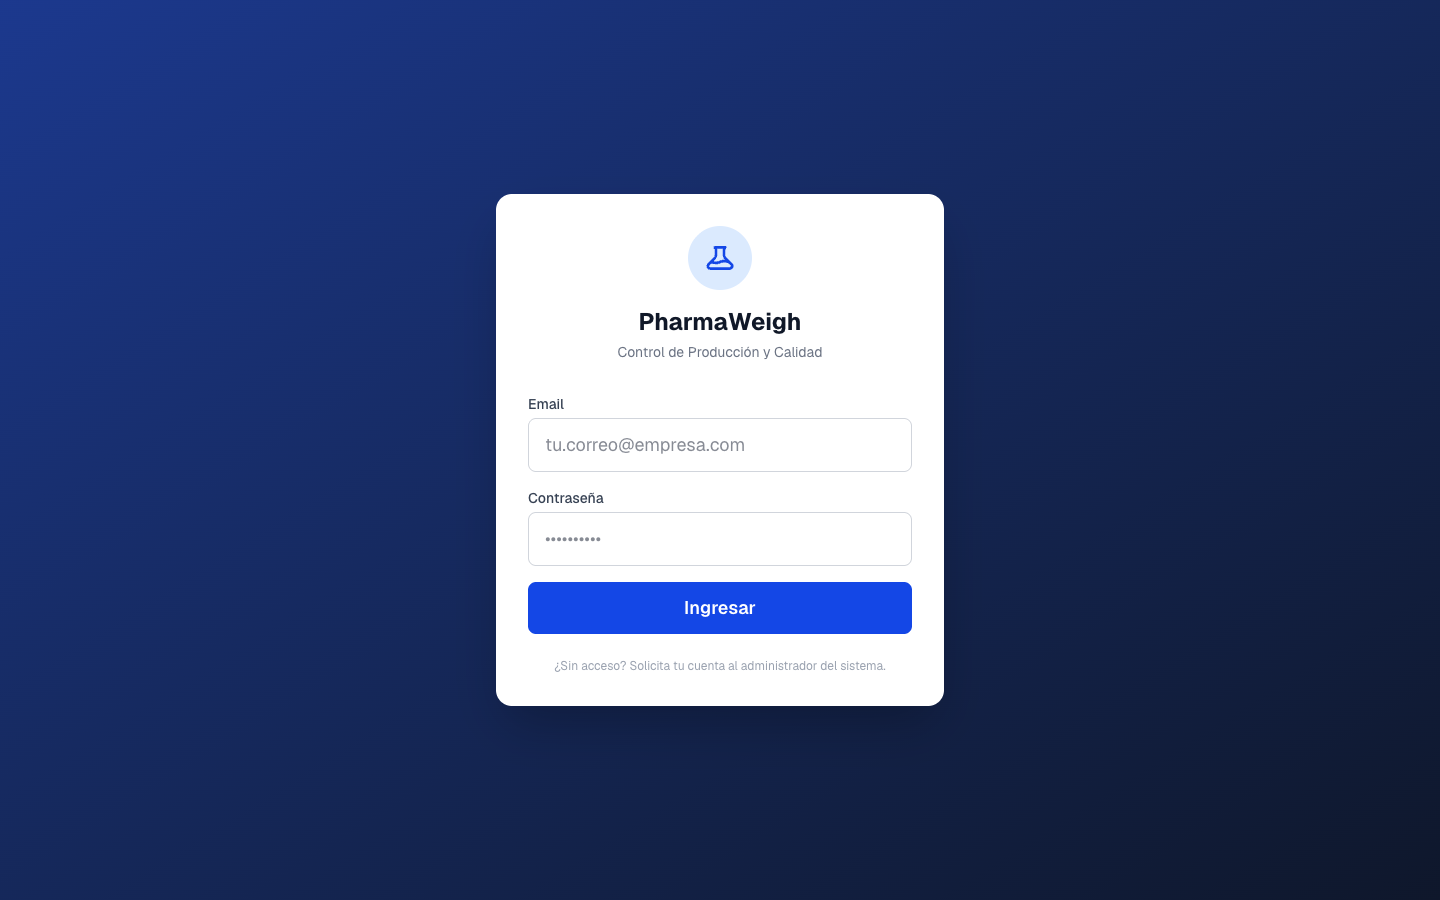
\includegraphics[width=0.85\linewidth]{capturas/01_login.png}}\\[3pt]
{\footnotesize\color{gristexto}Pantalla de inicio de sesión. Ingresa tu email y contraseña.}
\end{center}

Como \textbf{Auditor}, tienes acceso de \textbf{solo lectura} a todos los
registros del sistema. No puedes crear, modificar ni eliminar nada.
Tu función es verificar el cumplimiento normativo y la trazabilidad.

\begin{cajaNota}
\textbf{Tu menú lateral muestra:} Dashboard, Órdenes (consulta), Dispensado
(consulta), Recetas (consulta), Inventario (consulta) y Auditoría.
No tienes acceso a Usuarios ni Códigos de Barras.
\end{cajaNota}

% =====================================================================
\seccion{2. Tu rol en la organización}

Como auditor, eres independiente del proceso de producción.
Tu función es \textbf{verificar} que todo se haya hecho correctamente:

\vspace{6pt}
\begin{center}
\begin{tikzpicture}[
    node distance=0.5cm and 1cm,
    every node/.style={font=\footnotesize},
    paso/.style={draw=pharmablue, fill=pharmablue!8, rounded corners=6pt,
        minimum width=2.2cm, minimum height=0.9cm, align=center, text width=2cm},
    tuyo/.style={draw=gristexto, fill=gray!15, rounded corners=6pt,
        minimum width=5cm, minimum height=1.2cm, align=center, text width=4.8cm,
        line width=1.5pt},
    flecha/.style={-{Stealth[length=5pt]}, thick, color=gristexto}
]
\node[paso] (des) {DESARROLLO\\Receta};
\node[paso, right=of des] (alm) {ALMACÉN\\Recepción};
\node[paso, right=of alm] (cal) {CALIDAD\\Aprobación};
\node[paso, right=of cal] (sup) {SUPERVISOR\\Orden};
\node[paso, right=of sup] (op) {OPERARIO\\Dispensado};
\draw[flecha] (des) -- (alm);
\draw[flecha] (alm) -- (cal);
\draw[flecha] (cal) -- (sup);
\draw[flecha] (sup) -- (op);

\node[tuyo, below=1.2cm of cal] (audit) {\textbf{AUDITOR}\\Verifica todo el proceso --- Solo lectura};
\draw[dashed, thick, color=gristexto] (audit.north west) -- (des.south);
\draw[dashed, thick, color=gristexto] (audit.north east) -- (op.south);
\end{tikzpicture}
\end{center}
\vspace{6pt}

\begin{cajaInfo}[Independencia del auditor]
El auditor \textbf{no participa} en ninguna etapa del proceso productivo.
Su acceso de solo lectura garantiza que no puede alterar registros ni
influir en las operaciones que está verificando.
\end{cajaInfo}

% =====================================================================
\newpage
\seccion{3. Dashboard}

\begin{center}
\fbox{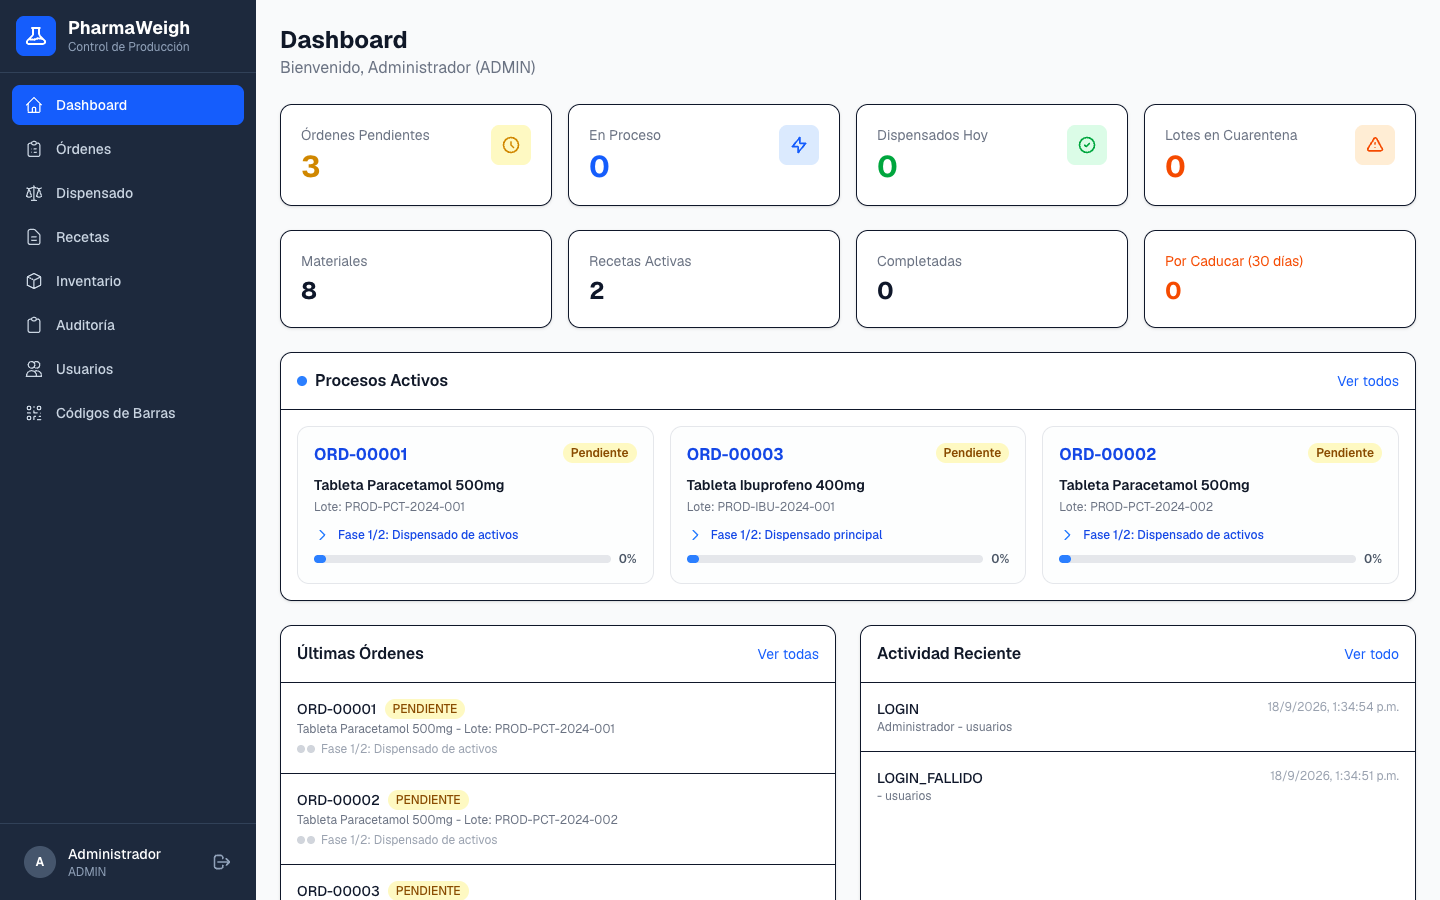
\includegraphics[width=0.92\linewidth]{capturas/03_dashboard.png}}\\[3pt]
{\footnotesize\color{gristexto}Dashboard principal con indicadores de producción y actividad reciente.}
\end{center}

El dashboard te da una vista rápida del estado general:
\begin{itemize}
    \item \textbf{Órdenes Pendientes vs.\ Completadas:} ¿hay cuellos de botella?
    \item \textbf{Lotes en Cuarentena:} ¿se están aprobando a tiempo?
    \item \textbf{Actividad Reciente:} últimas acciones --- ¿hay patrones inusuales?
    \item \textbf{Por Caducar (30 días):} ¿se está manejando bien la rotación?
\end{itemize}

% =====================================================================
\seccion{4. Módulo de auditoría}

Este es \textbf{tu módulo principal}. Aquí encuentras el registro inmutable
de todas las acciones del sistema.

\begin{center}
\fbox{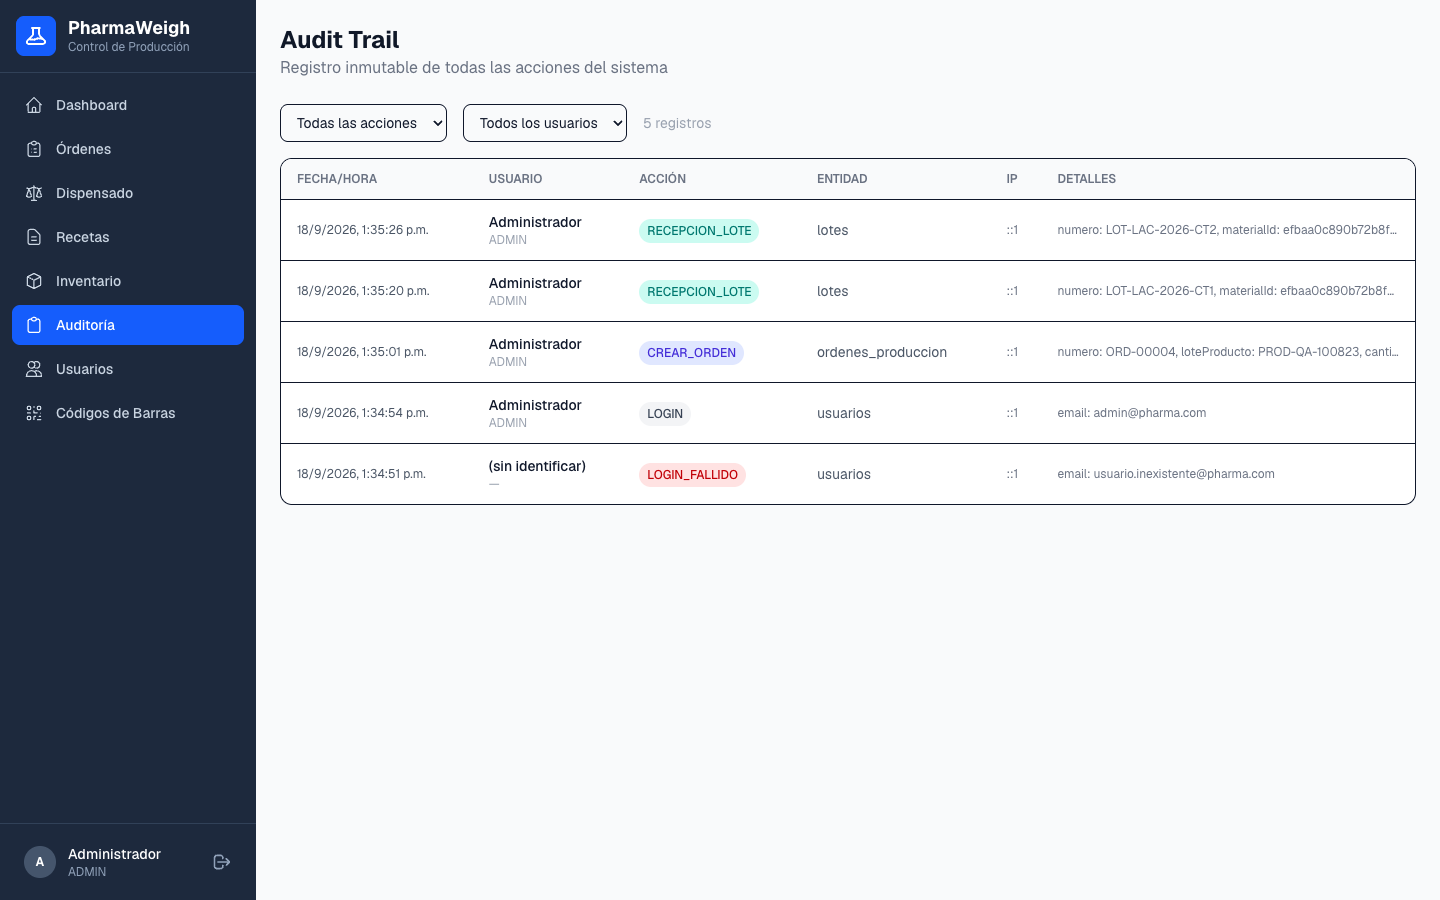
\includegraphics[width=0.92\linewidth]{capturas/17_auditoria.png}}\\[3pt]
{\footnotesize\color{gristexto}Log de auditoría: registro inmutable con filtros por acción y usuario.}
\end{center}

\subseccion{4.1 Información de cada registro}

Cada entrada de auditoría contiene:

\begin{center}
\begin{tabularx}{\linewidth}{@{}l >{\raggedright\arraybackslash}X@{}}
\toprule
\textbf{Campo} & \textbf{Descripción} \\
\midrule
Fecha y hora     & Timestamp exacto del evento (zona horaria del servidor) \\
Usuario          & Nombre del usuario que ejecutó la acción \\
Rol              & Rol del usuario al momento de la acción \\
Acción           & Tipo de evento (color codificado) \\
Entidad          & Tabla afectada (usuarios, lotes, recetas, etc.) \\
Detalles         & Datos específicos del cambio (JSON expandible) \\
\bottomrule
\end{tabularx}
\end{center}

\subseccion{4.2 Tipos de acciones registradas}

\begin{center}
\begin{tabularx}{\linewidth}{@{}l >{\raggedright\arraybackslash}X@{}}
\toprule
\textbf{Acción} & \textbf{Se registra cuando...} \\
\midrule
LOGIN                 & Un usuario ingresa al sistema \\
CREAR\_MATERIAL       & Se registra una nueva materia prima \\
RECEPCION\_LOTE       & Se recibe un lote de materia prima \\
CAMBIAR\_ESTADO\_LOTE & Se aprueba, rechaza o modifica el estado de un lote \\
CREAR\_RECETA         & Se crea una nueva formulación \\
CREAR\_ORDEN          & Se genera una orden de producción \\
DISPENSAR             & Un operario pesa un material \\
FIRMAR\_FASE          & Un supervisor/calidad firma electrónicamente una fase \\
COMPLETAR\_DISPENSADO & Se cierra una orden de dispensado \\
CREAR\_USUARIO        & Se crea una nueva cuenta de usuario \\
\bottomrule
\end{tabularx}
\end{center}

\newpage
\subseccion{4.3 Filtros de búsqueda}

Puedes filtrar el log por:
\begin{itemize}
    \item \campo{Por acción:} selecciona un tipo específico de evento.
    \item \campo{Por usuario:} filtra las acciones de un usuario particular.
\end{itemize}

\subseccion{4.4 Consultas clave para auditoría}

\begin{center}
\begin{tabularx}{\linewidth}{@{}l >{\raggedright\arraybackslash}X@{}}
\toprule
\textbf{Pregunta de auditoría} & \textbf{Cómo encontrar la respuesta} \\
\midrule
¿Quién aprobó este lote?        & Filtrar por CAMBIAR\_ESTADO\_LOTE, buscar el lote \\
¿Cuánto pesó el operario?       & Filtrar por DISPENSAR --- ver peso real vs.\ target \\
¿Quién firmó esta orden?        & Filtrar por FIRMAR\_FASE --- ver nombre del firmante \\
¿A qué hora se dispensó?        & Filtrar por DISPENSAR --- columna de timestamp \\
¿Quién creó esta receta?        & Filtrar por CREAR\_RECETA --- ver usuario y fecha \\
¿Quién creó este usuario?       & Filtrar por CREAR\_USUARIO --- ver quién y cuándo \\
\bottomrule
\end{tabularx}
\end{center}

% =====================================================================
\seccion{5. Verificación de cumplimiento 21 CFR Part 11}

El sistema está diseñado para cumplir con la regulación FDA para registros
y firmas electrónicas. Como auditor, verifica estos puntos:

\subseccion{5.1 Checklist de verificación}

\begin{center}
\begin{tabularx}{\linewidth}{@{}l l >{\raggedright\arraybackslash}X@{}}
\toprule
\textbf{Requisito} & \textbf{¿Cumple?} & \textbf{Evidencia en PharmaWeigh} \\
\midrule
Registros electrónicos & \semaverde & Toda acción genera registro con timestamp \\
Firmas electrónicas    & \semaverde & Email + contraseña del firmante \\
Audit trail            & \semaverde & Log inmutable, no editable, no borrable \\
Control de acceso      & \semaverde & 7 roles con permisos diferenciados \\
Integridad de datos    & \semaverde & PostgreSQL con transacciones ACID \\
Trazabilidad completa  & \semaverde & Material $\rightarrow$ Lote $\rightarrow$ Orden $\rightarrow$ Operario $\rightarrow$ Firma \\
Segregación de funciones & \semaverde & Quien pesa no puede firmar su propio trabajo \\
\bottomrule
\end{tabularx}
\end{center}

\begin{cajaInfo}[Cadena de trazabilidad]
Para cualquier producto terminado, puedes rastrear:
\begin{enumerate}
    \item \textbf{Receta} usada (quién la creó, cuándo)
    \item \textbf{Orden} de producción (quién la generó)
    \item \textbf{Lotes} de materia prima usados (proveedor, fecha, quién aprobó)
    \item \textbf{Operario} que dispensó (peso real de cada ingrediente)
    \item \textbf{Firma} de supervisión (quién firmó, cuándo)
\end{enumerate}
\end{cajaInfo}

% =====================================================================
\newpage
\seccion{6. Consultar recetas}

Desde \menu{Recetas} puedes verificar las formulaciones registradas:

\begin{center}
\fbox{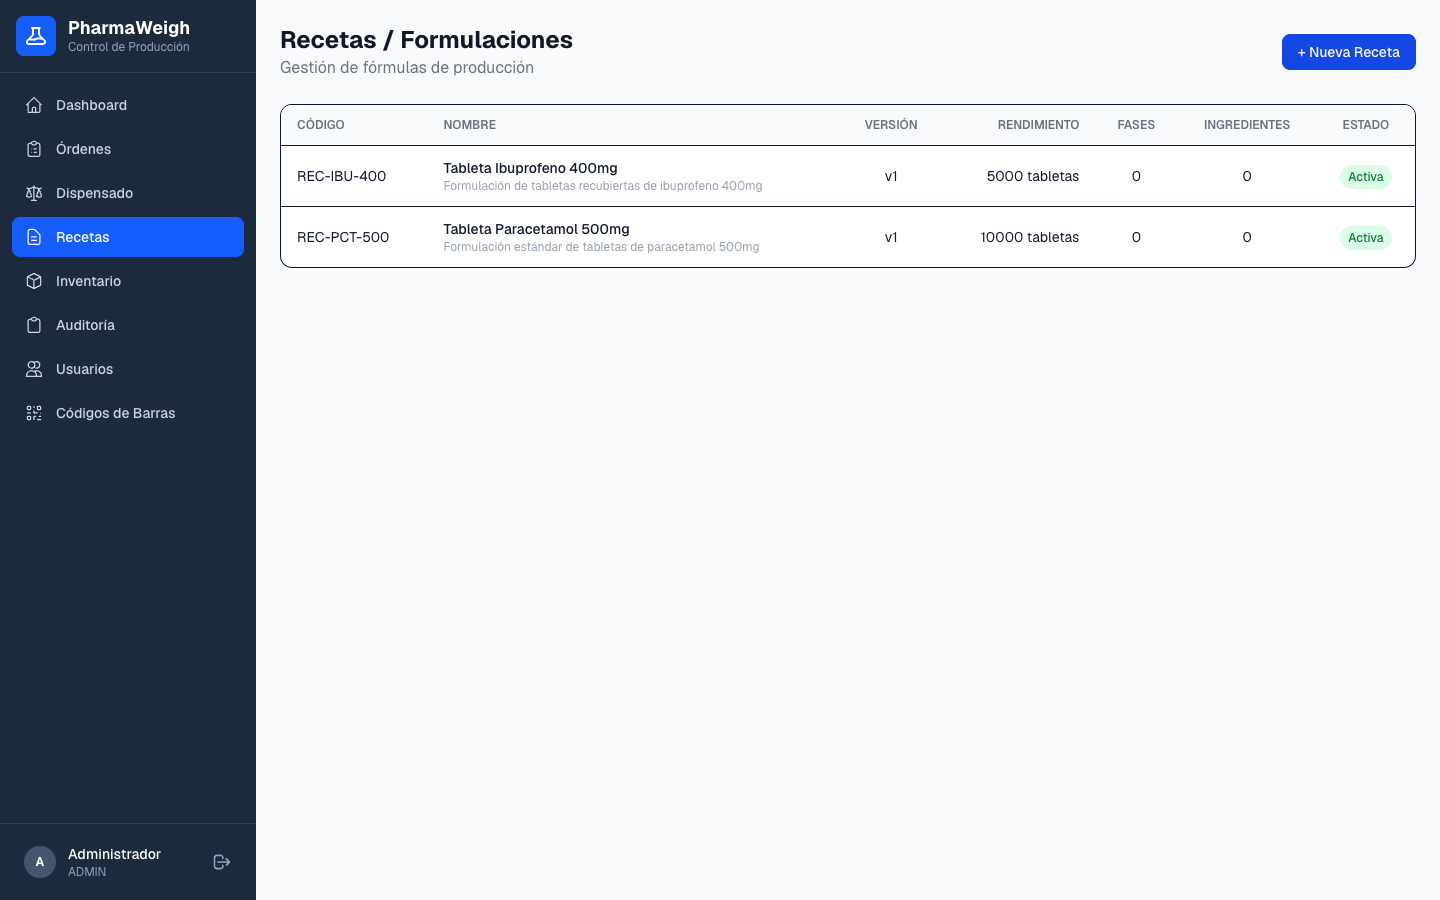
\includegraphics[width=0.92\linewidth]{capturas/12_recetas.png}}\\[3pt]
{\footnotesize\color{gristexto}Lista de recetas con código, nombre, versión, rendimiento e ingredientes.}
\end{center}

Verifica que:
\begin{itemize}
    \item Las recetas tengan tolerancias definidas para cada ingrediente.
    \item Los materiales peligrosos estén marcados correctamente.
    \item Las instrucciones para el operario sean claras y específicas.
\end{itemize}

% =====================================================================
\seccion{7. Consultar inventario}

Desde \menu{Inventario} verifica el estado de materiales y lotes:

\begin{center}
\fbox{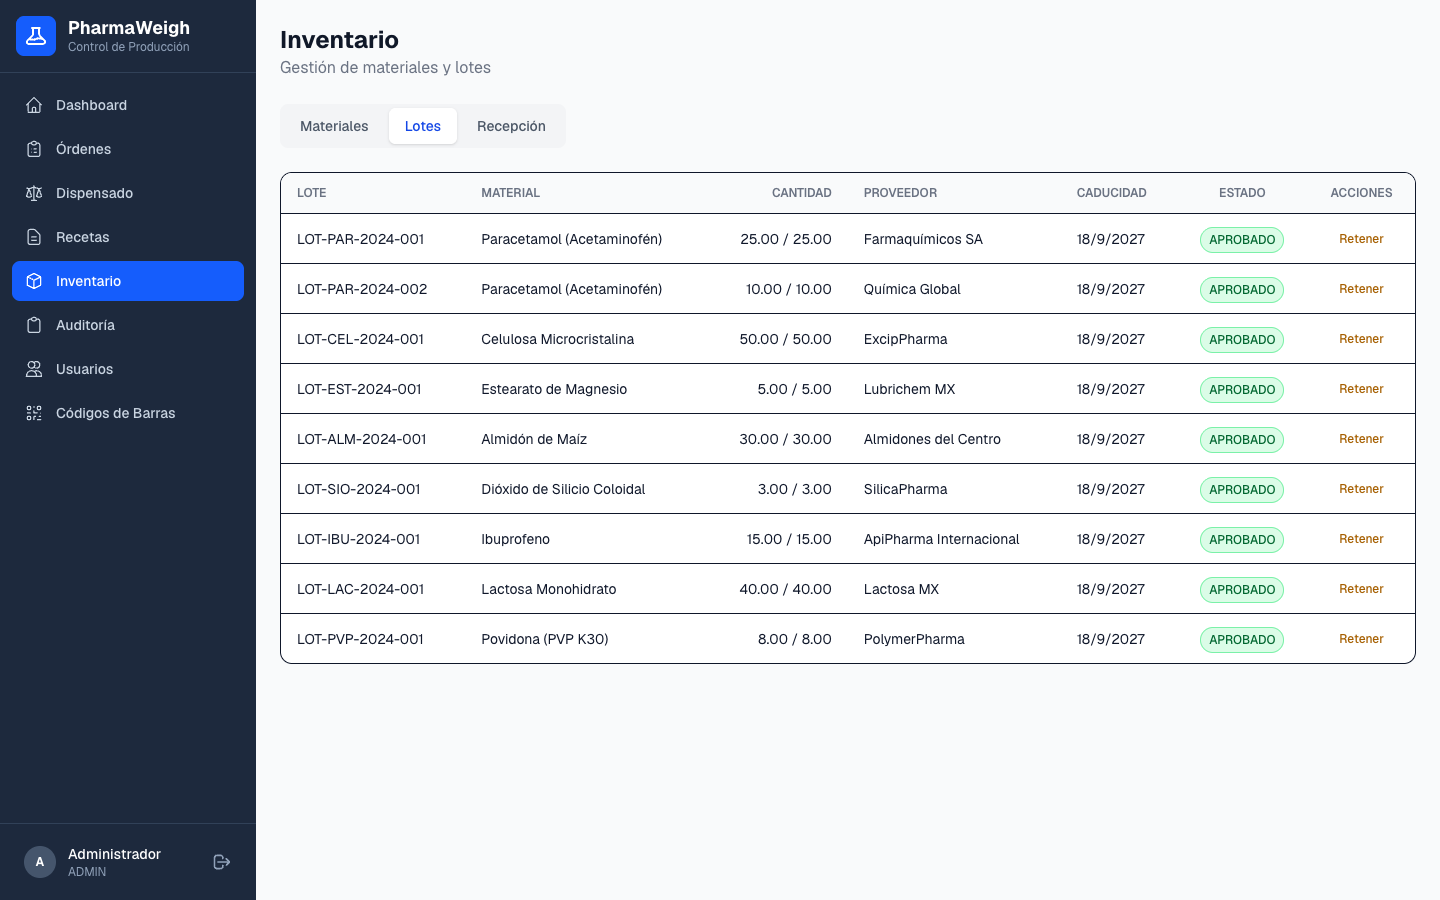
\includegraphics[width=0.92\linewidth]{capturas/15_inventario_lotes.png}}\\[3pt]
{\footnotesize\color{gristexto}Inventario de lotes con estado, cantidad, proveedor y caducidad.}
\end{center}

Puntos clave para auditoría:
\begin{itemize}
    \item ¿Hay lotes en cuarentena sin aprobar por más de 48 horas?
    \item ¿Hay lotes aprobados próximos a caducar sin usar?
    \item ¿Los proveedores son consistentes con los aprobados?
\end{itemize}

% =====================================================================
\seccion{8. Consultar órdenes}

\begin{center}
\fbox{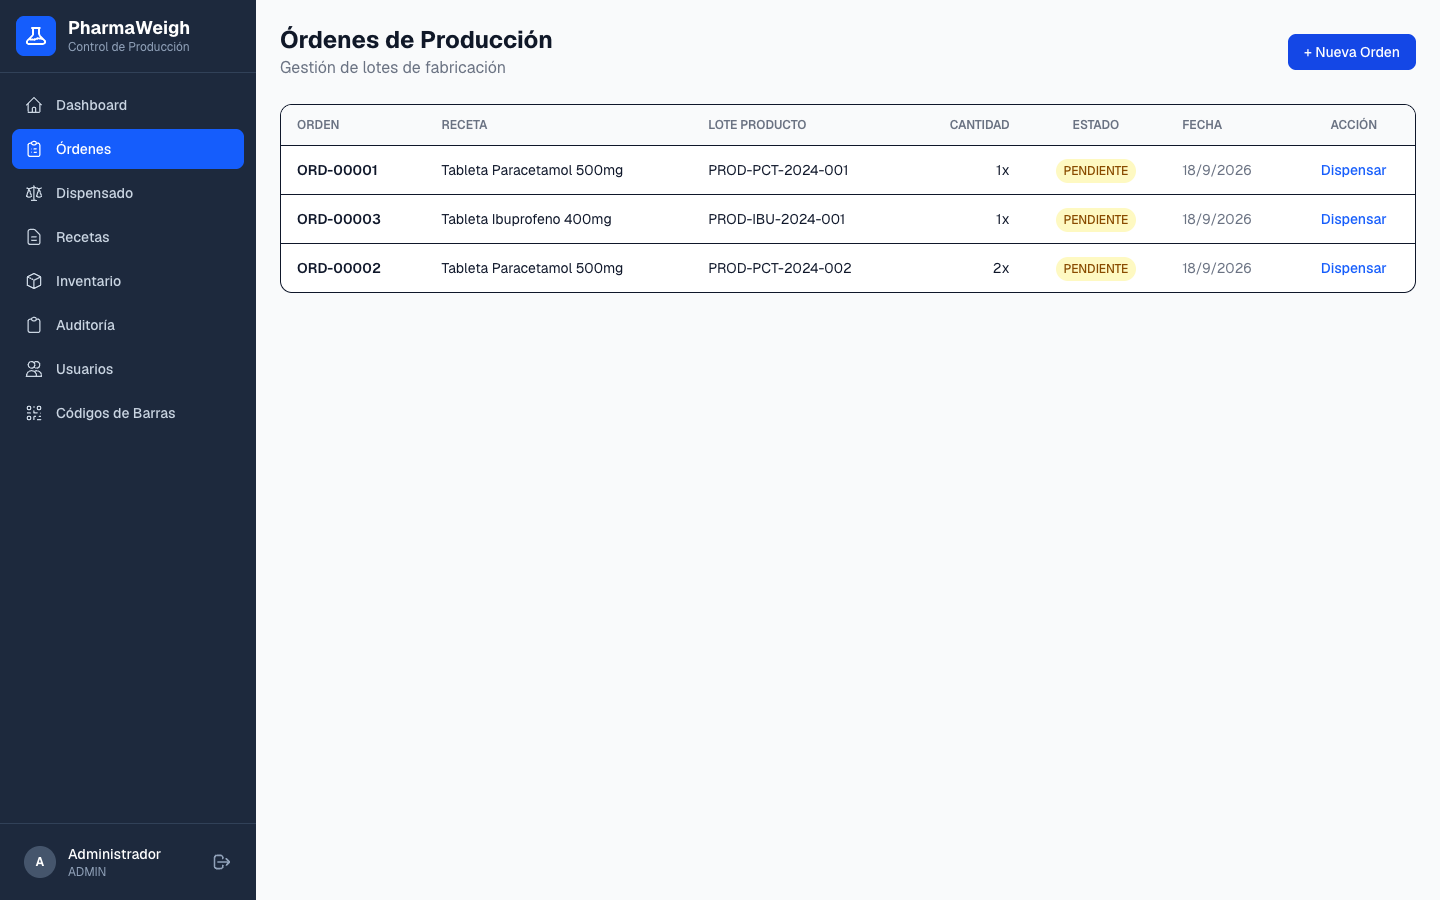
\includegraphics[width=0.92\linewidth]{capturas/04_ordenes.png}}\\[3pt]
{\footnotesize\color{gristexto}Órdenes de producción con estado, receta y prioridad.}
\end{center}

Verifica que:
\begin{itemize}
    \item Las órdenes completadas tengan firma electrónica.
    \item No haya órdenes atascadas en estado ``EN PROCESO'' por tiempo excesivo.
    \item Las prioridades se estén respetando (urgentes primero).
\end{itemize}

% =====================================================================
\newpage
\seccion{9. Equipo de la estación de pesaje}

Para tus inspecciones físicas, conoce el equipo del área de dispensado:

\subseccion{9.1 Báscula (ingreso manual)}

\begin{center}
\begin{tikzpicture}[
    every node/.style={font=\small}
]
\draw[fill=gray!10, draw=gray, rounded corners=4pt, line width=1pt]
    (0,0) rectangle (5,3);
\draw[fill=white, draw=gray!60, rounded corners=2pt]
    (0.5,1.5) rectangle (4.5,2.7);
\node[font=\Large\bfseries\color{pharmaazul}] at (2.5,2.1) {5.023 kg};
\node[font=\footnotesize\color{gristexto}] at (2.5,0.7) {Báscula de pesaje};

\draw[-{Stealth[length=6pt]}, thick, color=pharmablue] (5.3,1.5) -- (7,1.5)
    node[midway, above, font=\footnotesize\color{gristexto}] {Lectura visual};
\node[draw=pharmablue, fill=pharmablue!5, rounded corners=4pt,
    minimum width=2.5cm, minimum height=1.5cm, align=center]
    at (8.5,1.5) {Ingreso manual\\en PharmaWeigh\\(no conectada)};
\end{tikzpicture}
\end{center}

\begin{cajaNota}
La báscula \textbf{no está conectada} al sistema. El operario lee el peso y lo
ingresa manualmente. Esto es un punto de control importante: durante inspecciones,
puedes cruzar el peso registrado en el sistema contra la calibración de la báscula.
\end{cajaNota}

\subseccion{9.2 Pistola láser (lector de código de barras)}

\begin{center}
\begin{tikzpicture}[
    every node/.style={font=\small}
]
\draw[fill=gray!15, draw=gray, rounded corners=3pt, line width=1pt]
    (0,0.5) -- (1.5,0.5) -- (2,1) -- (2,2.5) -- (1.5,3) -- (0,3) -- cycle;
\draw[fill=red!30, draw=red!60] (2,1.7) -- (3.5,1.2) -- (3.5,1.5) -- (2,2) -- cycle;
\node[font=\footnotesize\color{gristexto}] at (1,0) {Pistola láser USB};

\draw[-{Stealth[length=6pt]}, thick, color=pharmablue] (4.2,1.5) -- (5.5,1.5);

\draw[fill=white, draw=gray, rounded corners=2pt]
    (5.8,0.3) rectangle (9.2,2.7);
\foreach \x in {6.1,6.3,6.4,6.7,6.8,7.1,7.2,7.4,7.7,7.8,8.0,8.2,8.4,8.6,8.8} {
    \draw[line width=1.2pt] (\x,0.8) -- (\x,2.2);
}
\node[font=\ttfamily\footnotesize] at (7.5,0.5) {LOT-PAR-2024-001};
\end{tikzpicture}
\end{center}

La pistola valida automáticamente: material correcto, lote aprobado,
no caducado y con stock suficiente. Este es un control crítico del sistema.

% =====================================================================
\seccion{10. Preguntas frecuentes}

\subseccion{¿Puedo modificar algún registro?}
No. Tu acceso es de \textbf{solo lectura}. No puedes crear, editar ni eliminar
ningún dato del sistema.

\subseccion{¿Puedo exportar el log de auditoría?}
Actualmente puedes consultar todo en pantalla con filtros. Para reportes
formales, toma capturas de pantalla o solicita al administrador.

\subseccion{¿El log de auditoría puede ser alterado?}
No. Los registros son inmutables. No existe función para editar ni borrar
entradas del log, ni siquiera para el administrador.

\subseccion{¿Cómo verifico la segregación de funciones?}
En la auditoría, para cada orden de dispensado, verifica que:
\begin{itemize}
    \item El usuario que pesó (DISPENSAR) sea diferente al que firmó (FIRMAR\_FASE).
    \item El usuario que creó la receta sea diferente al que la ejecutó.
    \item Quien aprobó el lote sea diferente al almacenista que lo recibió.
\end{itemize}


\end{document}
